\subsection{Distortion viewing techniques for 3-dimensional data}
\begin{frame}\frametitle{\emph{Distortion viewing techniques for 3-dimensional data} \cite{857608}} 
\begin{itemize}
	\item Apresenta o conceito de \emph{Visual Access Distortion}:
	\begin{itemize}
		\item Aumentar o foco e assim permitir uma vis�o mais detalhada.
		\item Permitir a rota��o do objeto 3D.
		\item \alert{Manter um caminho visual limpo do observador at� o foco.}
	\end{itemize}
\end{itemize}
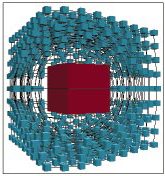
\includegraphics[height=100.0px]{img/cga97}
\end{frame}

\begin{frame}\frametitle{\emph{Distortion viewing techniques for 3-dimensional data} \cite{857608}} 
\begin{itemize}
	\item Para manter um caminho visual limpo do observador at� o foco, o artigo prop�e os seguintes passos:
	\begin{enumerate}
		\item Selecionar um ponto focal.
		\item Seja L um segmento de reta do ponto focal at� o observador.
		\item O vetor \textbf{d} ser� o menor vetor de um objeto \emph{O} at� o ponto mais pr�ximo \emph{P} na reta L.
		\begin{itemize}
			\item O vetor \textbf{d} ir� definir a dire��o em que o objeto \emph{O} deve seguir.
			\item O comprimento \textbf{$|d|$} ir� determinar a magnitude da distor��o dos objetos \emph{O}. A distor��o tamb�m � controlada por uma distribui��o gaussiana.
		\end{itemize}
	\end{enumerate}
\end{itemize}
\begin{center}
	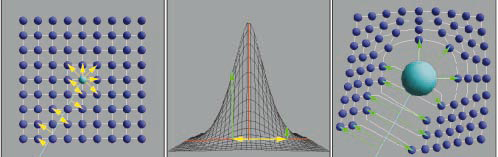
\includegraphics[height=50.0px]{img/cga972}
\end{center}
\end{frame}

\begin{frame}\frametitle{\emph{Distortion viewing techniques for 3-dimensional data} \cite{857608}} 
\begin{itemize}
	\item Os trabalhos seguintes aproveitaram a proposta de \cite{857608}:
	\begin{columns}[T]
	\begin{column}{5cm}
	\begin{itemize}
		\item \alert<1>{\emph{Integrating Expanding Annotations with a 3D Explosion Probe} \cite{23}}
		\item \alert<2>{\emph{Exploded Views for Volume Data} \cite{1187828}}
	\end{itemize}
	\vspace{3cm} 
	\end{column}
	\begin{column}{5cm}
	\begin{overprint}
		\includegraphics<1>[height=100.0px]{img/Integrating_Expanding_Annotations}
		\includegraphics<2>[height=100.0px]{img/bruckner-2006-EVV-Paper}
	\end{overprint}
	\end{column}
	\end{columns}
\end{itemize}
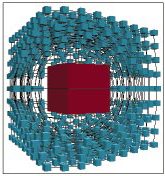
\includegraphics[height=100.0px]{img/cga97}
\end{frame}